The previous chapter addressed different aspects of a cooperative perception system conceptually. First, a uniform, expressive and extensible way to model traffic scenes for cooperative perception was proposed alongside an appropriate representation format for it. Different characteristics and benefits of 5G cellular networks were discussed before a high-level system architecture, involving a multitude of different modular software components, was elaborated. Eventually, a concept was presented on how to combine observations from different actors, while taking temporal delay and uncertainty into account. 
\par
\bigskip

The purpose of this chapter is to pick up the previously presented concepts and techniques and explain how they were implemented in software. This includes a discussion about various technological choices, the use of appropriate software design patterns and fundamental performance-related considerations. \Cref{fig:components_full} shows the component diagram from \cref{subsec:concept_design:components_overview} again, but now includes implementation-specific technologies in addition. It serves as a guideline for this chapter, as the implementation of each individual components is explained subsequently. 

\begin{figure}[h]
	\centering
	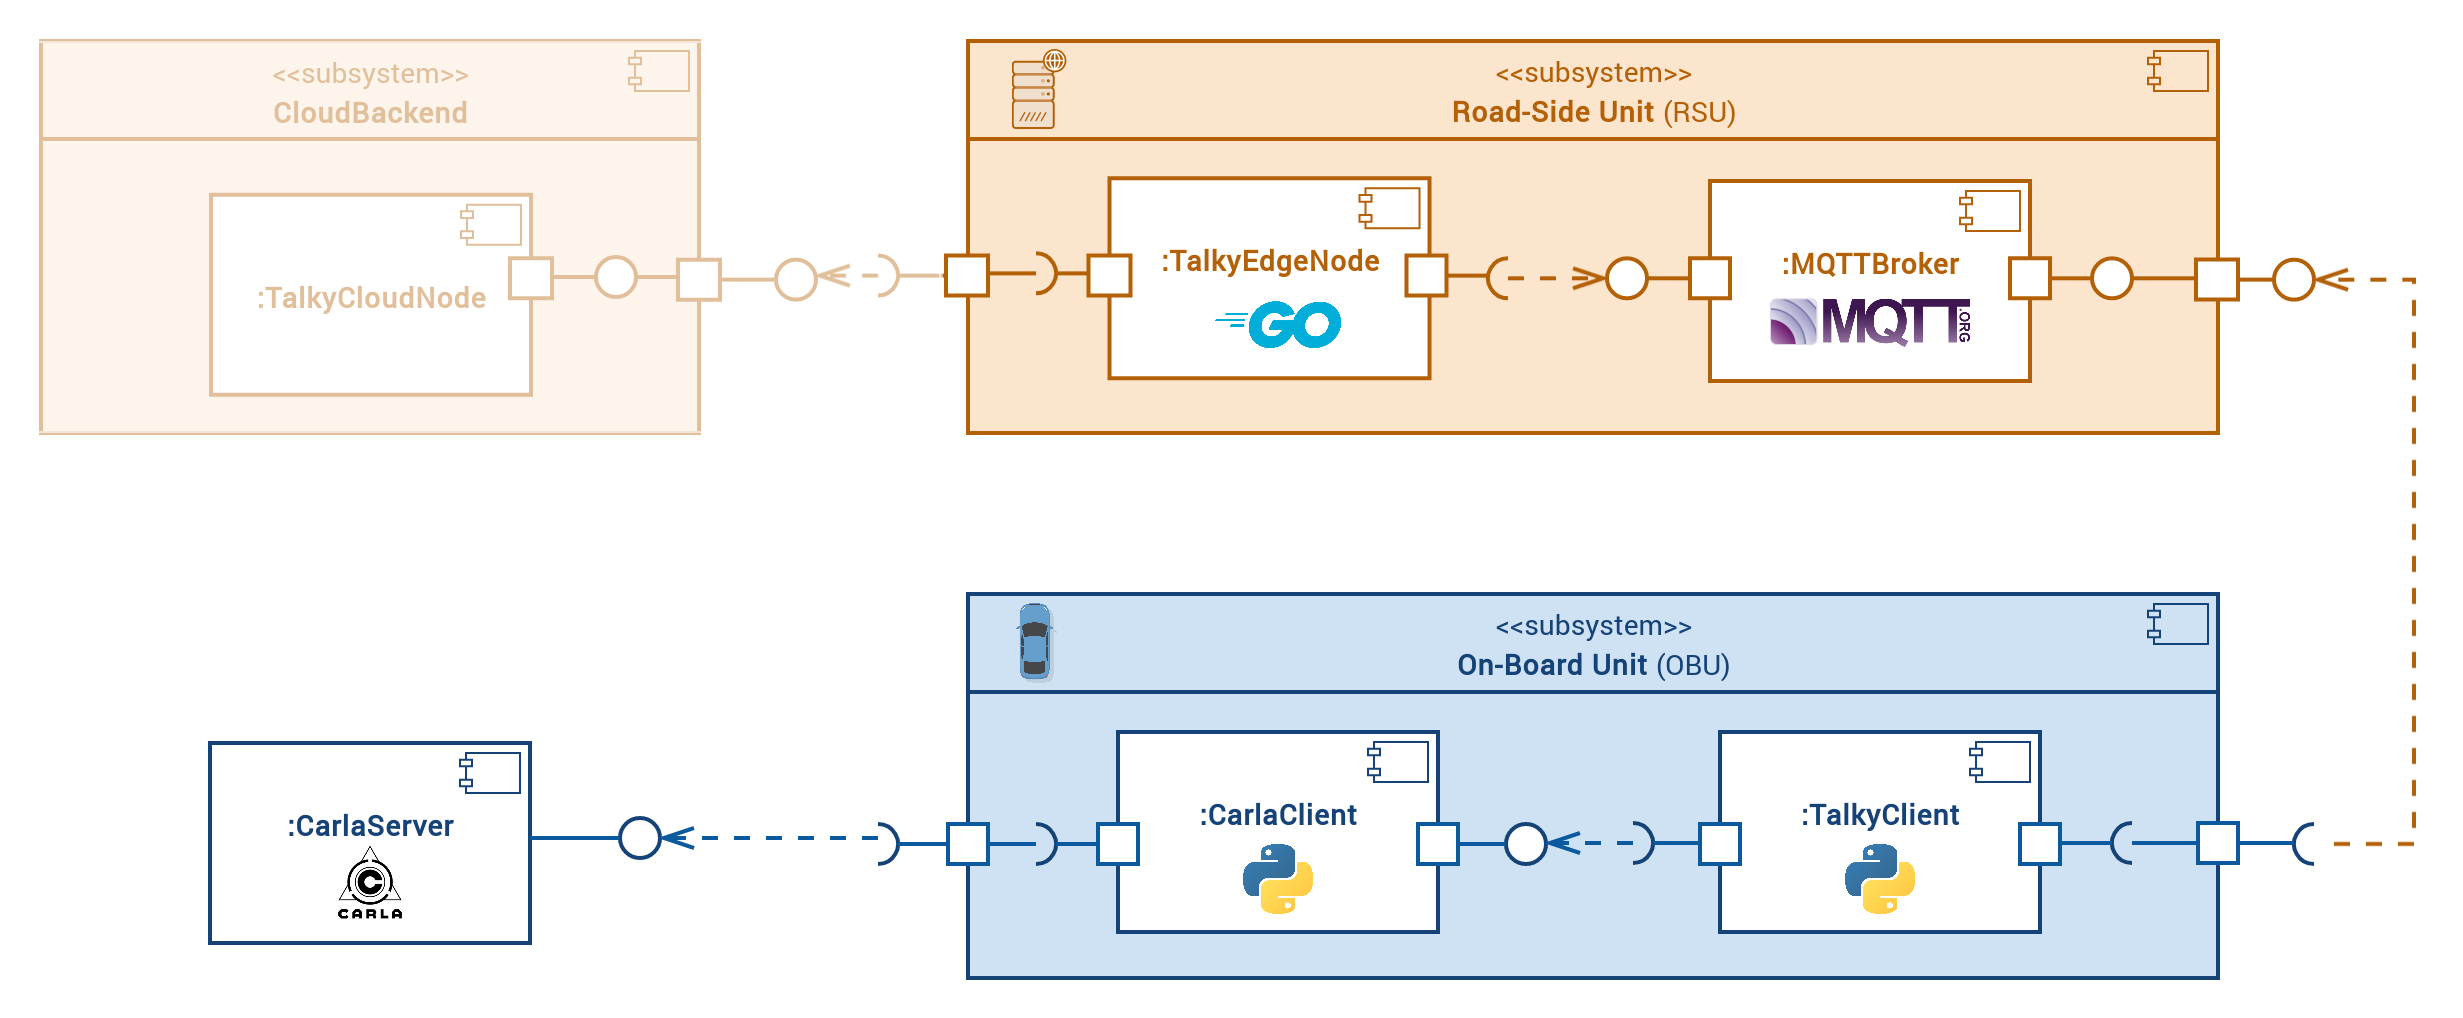
\includegraphics[width=1\linewidth]{98_images/components_full}
	\caption{UML Component Diagram – Implementation}
	\label{fig:components_full}
\end{figure}
\par
\bigskip

During the implementation process, design- and component principles presented in \cite{Martin2017} were followed with the purpose to develop clean, modular and maintainable software components.

\section{Meta Model, Representation- \& Message Format}
\label{sec:implementation:meta_model_representation_message_format}

\subsection{Object-Oriented Model}
\label{subsec:implementation:object_oriented_model}
The meta model presented in \cref{sec:concept_design:environment_modeling_state_representation} is a probabilistic entity relationship model, i.e. essentially an ER model that is extended to incorporate a notion of structural- and relational uncertainty. As explained earlier, it can be viewed as a graph in which entities relate to other entities or attributes with a certain probability or confidence. Accordingly, the graph can also be represented as a collection of quadruples $r_i = \langle \textit{subject}, \textit{predicate}, \textit{object}, \alpha \rangle$ with $\alpha$ being the corresponding confidence factor. 

In code, this graphical structure is implemented as a composition of pure object-oriented classes. As Python was chosen as the primary programming language, the built-in Python class system is employed. Each type of entity corresponds to a certain class, which inherits from an abstract \texttt{Entity} class. Relations (both entity-entity and entity-attribute) are implemented as sub-classes of an abstract \texttt{Relation} class, which is attached to its object as a class member and holds members for its object (either a literal attribute or another entity) and the corresponding confidence. Deviating from the quadruple structure, an exception is introduced for convenience to additionally allow for the specification of attributes without uncertainty as well. Such are simply implemented as ordinary class members and should only be used to encode meta data, but not actual observations. Listing \ref{lst:class_example} depicts a simplified example of this modeling schema.

Most of the entities, attributes and relations from the final model, presented in \cref{subsec:concept_design:the_final_model}, were implemented according to the above class schema and encapsulated as a re-usable Python library.

\begin{samepage}
\inputminted[fontsize=\footnotesize]{python}{97_listings/class_example.py}
\captionof{listing}{Example Implementation of PER Entities and Relations}
\label{lst:class_example}
\end{samepage}

\par
\medskip
One might wonder why a cell's \texttt{hash} attribute is declared as an integer data type, even though QuadKeys (cf. \cref{subsec:background:quadkeys}) are strings. This is due to the fact that the implementation takes advantage of an optimization in representing QuadKeys. In addition to using ASCII encoding, where every character is one byte, QuadKeys can also be represented as integers for better space efficiency. In integer representation, the length of a key is only limited by the underlying data type (usually 64 bits). The size complexity is then given as $O(1)$ compared to $O(n)$ with strings ($n$ being the precision level, or key length).

\subsection{Serialization Format}
\label{subsec:implementation:serialization_format}
The object-oriented schema presented in the previous section is used as a module throughout all related Python code. However, instances of these classes only exist within the scope of a certain process. In order to transfer these information across different programs, which are potentially even written in different programming languages, a language-agnostic, commonly understandable format is needed. In technical terms, objects must be \textit{serialized}, then transmitted and \textit{deserialized} again afterwards. Multiple common serialization formats exist, which differ in certain properties. Some are text-based and potentially also human-readable, others are binary formats and only understandable by machines. While text-based formats are generally more common and easier to work with, \cref{subsec:concept_design:messaging_further_considerations} motivated the use of binary formats for performance- and efficiency-critical applications like CP.

Common binary serialization formats include Apache Thrift\footnote{\url{https://thrift.apache.org/}}, Cap'n'Proto\footnote{\url{https://capnproto.org/}},  Flatbuffers\footnote{\url{https://google.github.io/flatbuffers/}} and Protocol Buffers\footnote{\url{https://developers.google.com/protocol-buffers/}} (Protobuf). Most of them follow the principle of first defining a static class (or message) schema, which is then compiled to language-specific code to be used by different applications equally. During serialization, objects and attributes are condensed to an efficient binary representation, which can usually be accessed as a byte stream or -array subsequently. Since all of these formats are relatively similar, a detailed comparison and evaluation is out of scope.

In a first iteration \textbf{Cap'n'Proto} was used. Reasons for this decision included the high serialization performance claimed on the authors' website and the framework's novelty. However, as this work progressed, it became clear that serialization was a major performance bottleneck. In search of alternatives to Cap'n'Proto a brief evaluation\footnote{\url{https://github.com/n1try/talkycars-thesis/tree/master/src/evaluation/serialization}} revealed superior performance of \textbf{Protocol Buffers} format in comparison. In a simplified example, Protobuf was able to serialize \SI{7490}{messages\per\second} on average, compared to \SI{4129}{messages\per\second} with Cap'n'Proto (see \cref{sec:appendix:evaluation_results:serialization_benchmark}). Moreover, the average message size with Protobuf appeared to be up to $\sim$ 47 \% smaller for the same payload. The benchmarking was done using the Go programming language, Google's reference implementation of Protobuf for Go and the most common third-party open-source Go implementation of Cap'n'Proto\footnote{\url{https://github.com/capnproto/go-capnproto2}}. 

The performance improvement of $\sim$ 25 \% and potential size decrease of up to 47 \% led to the decision to refactor existing code and use Protocol Buffers for serialization over the course of this work.

Listing \ref{lst:serialization_schema_examples} gives an example for a simplified message schema definition in Protobuf and Cap'n'Proto, respectively.

\begin{figure}[!h]
	\begin{minipage}{0.5\textwidth}
		\centering
		\inputminted[fontsize=\footnotesize]{text}{97_listings/protobuf_snippet.proto}
	\end{minipage}
	\begin{minipage}{0.5\textwidth}
		\centering
		\inputminted[fontsize=\footnotesize]{text}{97_listings/capnp_snippet.capnp}
	\end{minipage}
	\captionof{listing}{Exemplary schema definitions in Protocol Buffers (left) and Cap'n'Proto (right)}
	\label{lst:serialization_schema_examples}
\end{figure}

\section{Simulation Environment}
\label{sec:implementation:simulation_environment}
Since the integration and evaluation with an autonomous driving simulator is one of the core goals of this thesis, an appropriate simulator must be chosen. A commonly used option is \textbf{SUMO}\footnote{\url{https://sumo.dlr.de/}} (Simulation of Urban Mobility). However, it focuses on traffic simulation and is not particularly built for in-depth simulations of autonomous driving. Instead, a variety of high-detail, photorealistic 3D simulators have established recently. The most commonly used options are the following.

\begin{itemize}
	\item \textbf{AirSim} by Microsoft \cite{airsim2017fsr} is an open-source ($\sim$ 9,300 GitHub stars, MIT license) 3D simulator for autonomous cars and drones based on the Unreal 4 game engine\footnote{\url{https://www.unrealengine.com}}. It has inherent support for Reinforcement Learning, allows to connect various kinds of external control devices and has a rich C++ and Python API to program it. Supported sensors are RGB camera, IMU, GPS, magnetometer, barometer, a custom distance sensor and LiDAR. 
	\item \textbf{Carla} \cite{Dosovitskiy17} is an independent open-source project (3,600 GitHub stars, MIT license). The 3D simulator is based on Unreal 4, has C++ and Python APIs and features a multitude of sensors, including RGB camera, depth camera, IMU, GPS and LiDAR. In addition, is has multi-agent support, i.e. allows multiple Python- or C++ clients to connect to the simulation server and also offers an integration with the Autoware AV stack\footnote{\url{https://www.autoware.ai/}}.
	\item \textbf{Carmaker}\footnote{\url{https://ipg-automotive.com/de/produkte-services/simulation-software/carmaker/}} by IPG Automotive GmbH is a proprietary 3D simulator featuring various integrations with hardware platforms and tools and offers an proprietary and a MATLAB programming interface.
	\item \textbf{LGSVL}\footnote{\url{https://www.lgsvlsimulator.com}} by LG is the latest of these 3D simulator projects, as development started in 2019. It is open-source ($\sim$ 700 GitHub stars, custom license), written in C\# and based on the Unity game engine\footnote{\url{https://unity3d.com}}, offers integrations with Autoware and Baidu's Apollo framework\footnote{\url{https://github.com/ApolloAuto/apollo}} and a Python API. Supported sensors include RGB camera, IMU, GPS, LiDAR, radar and CAN bus. While this project appears to be the most ambitious and promising one, it is still in quite early development and therefore partially unstable.
\end{itemize}

\begin{figure}
	\centering
	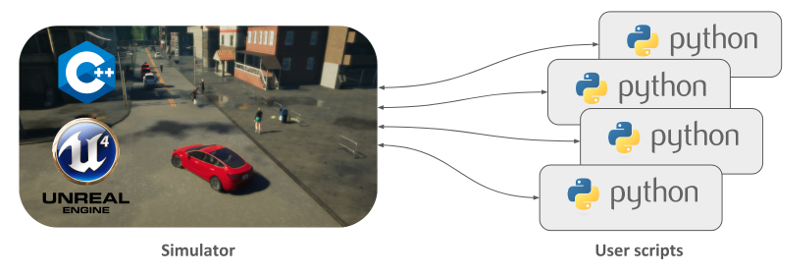
\includegraphics[width=0.8\linewidth]{98_images/carla_modules}
	\caption[Client-Server Schema in CARLA]{Client-Server Schema in CARLA \cite{CarlaContributors}}
	\label{fig:carla_modules}
\end{figure}

Mainly because of its extraordinarily rich and intuitive API, the large number of simulated sensors, the inherent multi-agent support an a vibrant open-source community Carla was chosen to be used as a simulation environment in this work. In addition to the features mentioned above, it also includes seven pre-defined high-detail maps, each of which represents a different scenario (e.g. urban or rural environments). Maps can be exported in the OpenDrive format and thanks to an integration with the RoadRunner\footnote{\url{https://www.vectorzero.io/}} software suite, custom maps can be created and imported easily. In addition to vehicles pedestrians and cyclists are supported as traffic participants as well and the open-source community has provided automated controllers and navigation scripts for each of these actor types. \Cref{fig:carla_modules} schematically outlines how a simulation running on a Carla server is controlled by one or multiple user scripts.

The screenshot in \cref{fig:carla_sceenshot_1} depicts an exemplary rural scene in Carla, involving two vehicles. It was recorded during an early development stage when the simulation client already supported to compute and render the occupancy grid corresponding to an ego vehicle's observations. Green cells are considered free, red cells are occupied and the state of blue cells is unknown, e.g. due to sensor noise or because they are out of sight.

\begin{figure}[h]
	\centering
	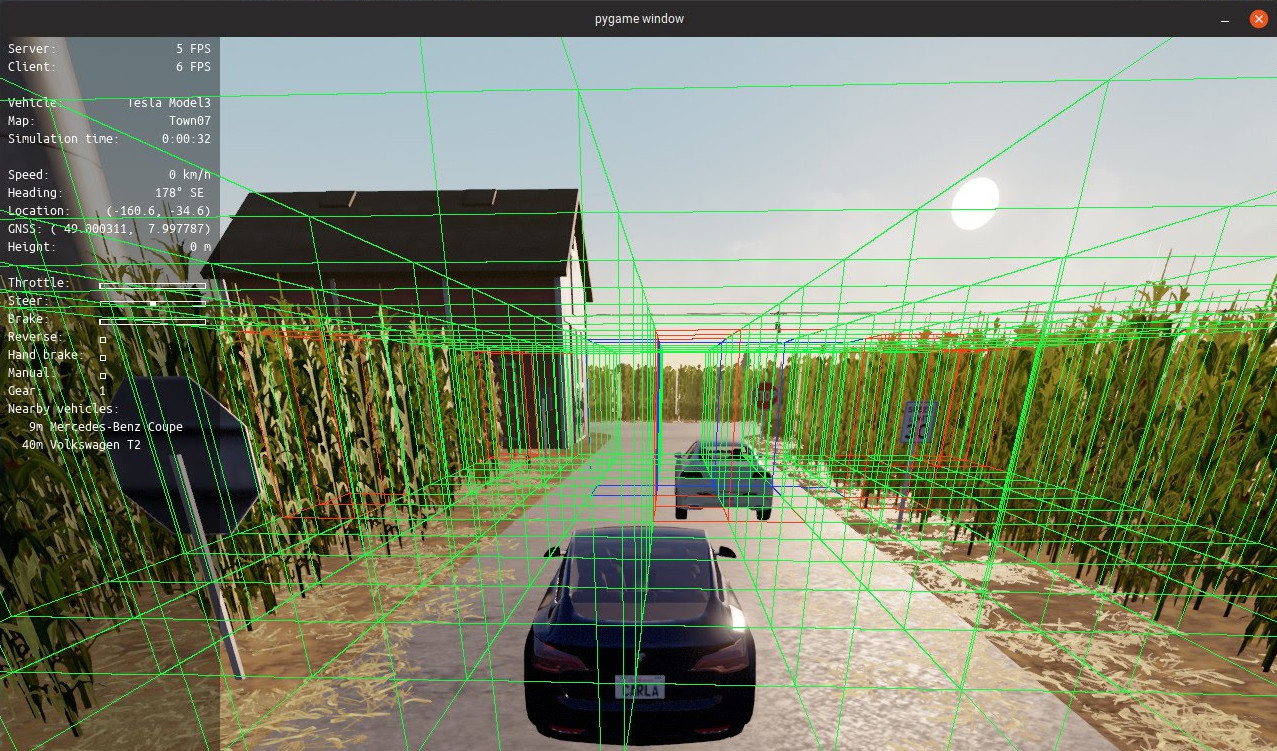
\includegraphics[width=0.9\linewidth]{98_images/carla_screenshot_1}
	\caption[Screenshot of an Exemplary Carla Scene]{Screenshot of an Exemplary Scene in Carla featuring two Vehicles and their Occupancy Grids}
	\label{fig:carla_sceenshot_1}
\end{figure}

\section{Server-Side Software Components}
\label{sec:implementation:server_side_software_components}
The following two sections discuss the implementation or integration process and respective details of the software components outlined in \cref{subsec:concept_design:components_overview}, starting with server-side components. These constitute the central processing instance that all participants within certain geographical area connect to and exchange information with. 

\subsection{Message Broker}
\label{subsec:implementation:message_broker}
A message broker's responsibility as part of a publish-subscribe (or messaging-based) software system is to maintain connections to all clients and receive and re-distribute their messages according to certain rules. Usually this involves the notion of a \textit{queue}, \textit{topic} or \textit{subject} as a basic routing mechanism for messages. Producers publish messages to a certain queue, which are then received by all consumers that had subscribed to that queue upfront. \Cref{fig:pubsub_topics} depicts this mechanism schematically. 

\begin{figure}
	\centering
	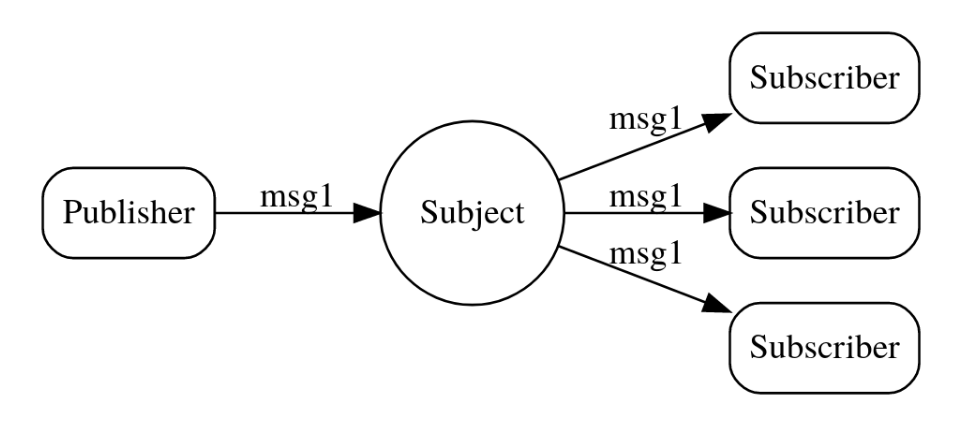
\includegraphics[width=0.65\linewidth]{98_images/pubsub}
	\caption[Schema of Publish-Subscribe Communication with Topics]{Schema of Publish-Subscribe Communication with Topics \cite{Collison2019}}
	\label{fig:pubsub_topics}
\end{figure}


A variety of messaging solutions and corresponding brokers already exist. When attempting to evaluate such, one has to distinguish between protocol and implementation. While the use of a messaging-based architecture has already been motivated in \cref{subsec:concept_design:messaging_further_considerations}, a concrete protocol and a corresponding software implementation need to be chosen in addition. 

Publish-subscribe protocols for data streaming include AMQP, the Apache Kafka messaging protocol\footnote{\url{https://kafka.apache.org/protocol}}, MQTT, NATS\footnote{\url{https://nats.io}} and more. Without conducting an in-depth evaluation of these alternatives, it can be concluded that each solution has various advantages and drawbacks with respect to different use cases. However, MQTT is the de-facto standard protocol for IoT applications and most widely spread. Accordingly, it has already proven effective and a variety of different proprietary and open-source implementations exist. Major benefits of MQTT include its low footprint in terms of messaging overhead and computational efficiency as well as the support for different quality of service (QoS) levels. QoS essentially allows the user to define the reliability of delivery for a certain message and has an impact on performance. Due to these benefits, MQTT is chosen as the pub/sub messaging protocol to be used for the present CP system. 

In addition to deciding for a protocol, a corresponding message broker implementation needs to be picked. For MQTT, a variety of different implementations in different programming languages and with varying feature sets exist. The most common ones are Apache ActiveMQ\footnote{\url{http://activemq.apache.org/}} (Java), HiveMQ\footnote{\url{https://www.hivemq.com/}} (Java), Mosca\footnote{\url{http://www.mosca.io/}} (JavaScript), Eclipse Mosquitto\footnote{\url{https://mosquitto.org/}} (C) and RabbitMQ\footnote{\url{http://rabbitmq.io/}} (Erlang). A basic performance comparison between different brokers was conducted by \cite{Mutsch2019} and the results are depicted in \cref{fig:mqtt_benchmarks}. Due to its good performance and easy setup procedure, Mosquitto was chosen for this work. However, since this thesis' implementation only uses standard MQTT features anyway, the broker could easily be switched by any other one, as it is a modular, stand-alone software component.

\begin{figure}
	\centering
	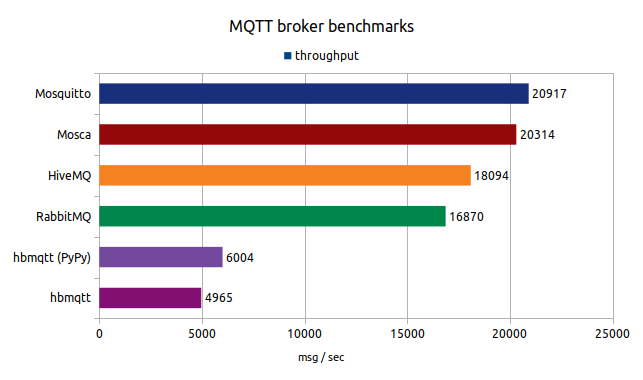
\includegraphics[width=0.9\linewidth]{98_images/mqtt_bench_2}
	\caption[Basic Performance Benchmark of Different MQTT Brokers]{Basic Performance Benchmark of Different MQTT Brokers \cite{Mutsch2019}}
	\label{fig:mqtt_benchmarks}
\end{figure}

\subsection{Talky Fusion Node}
\label{subsec:implementation:edge_side_fusion_node}
The second server-side component, which is deployed "'on the edge"', is the fusion node. While the message broker only acts as an intermediary, the fusion node is a core component of the proposed CP system. It is responsible for the aggregation of all its connected clients' (vehicles, etc.) observations. It is realized as a stand-alone software component and, in a first iteration, using the Python programming language. However, after some initial evaluations it turned out that Python as a dynamically typed, interpreted language was too slow to perform fusion for multiple clients at a reasonable update rate. As a consequence, a second iteration re-implemented the fusion node in Go, which yielded a performance improvement of up to two orders of magnitude. Due to a high degree of modularity, encapsulation and separation of concerns (cf. \cite{Martin2017}) the rewriting could be done with comparatively low effort.

The program relies on third-party open-source libraries  with MIT-, BSD-3- and EPL-1.0 licenses.
\par
\bigskip

The fusion algorithm as a core part of this component is modelled after the formal definitions described in \cref{sec:concept_design:fusion} and implemented to use multi-threading for parallelization, facilitated by Goroutines\footnote{\url{https://tour.golang.org/concurrency/1}} and Go channels. Messages are received via MQTT from the message broker using a subscription to a single topic, which all incoming observations are published to. Received messages are temporarily stored in an internal queue, from which they are picked up during the next fusion iteration. In line with the principle of periodic push, the fusion algorithm is executed at a configurable constant rate, e.g. \SI{10}{\hertz}. As part of an iteration, it fetches all observations from the queue, which are not older than a certain configurable threshold, e.g. one second. In a fusion procedure of $O(n*m*k)$ time complexity ($n \approx |\textit{cells}|, m \approx |\textit{observers}|, k \approx |\textit{observations per observer}|$), the occupancy grids are merged into a single one, which is subsequently split into type 2 tiles (see \cref{subsec:concept_design:geographical_partitioning}) and published to their respective MQTT topics periodically.

For instance, assume a vehicle is at position \texttt{120203233230313123011210}, $\lambda_2 = 19$ and $\lambda_3 = 16$. In that case, the current fusion node will be configured to be responsible for \texttt{1202032332303131} and the the vehicle will be subscribe to all of its surrounding level 19 tiles, including \texttt{1202032332303131230}. For this tile, among others, it will receive fused grids that were previously – ideally only few milliseconds ago – published by the fusion node.
\par
\bigskip

As mentioned earlier, the fusion node is implemented as a stand-alone software component contained in a single executable file and can be executed as such without additional dependencies. Required program arguments include the message broker's address and port and the type 3 QuadKey of the tile, which this node is supposed to be responsible for. Further parameters, including the maximum observation age, the fusion rate, MQTT topic and QoS and more can be specified via an additional configuration file.

\subsection{Web Visualization}
\label{subsec:implementation:web_visualization}

This component was not presented in \cref{subsec:concept_design:components_overview} as part of the system as it is only used for development and debugging. Its purpose is to visually depict the output generated by the fusion node. Thanks to a uniform interface and a common message format specification, this visualization component could be easily implemented as a light-weight, stand-alone software component using Python. It subscribes to a desired MQTT topic to receive fused PER model instances and relays these occupancy grids to a web-frontend via a featured webserver using Websockets, where they are eventually displayed. The screenshot in \cref{fig:screenshot_web_node} depicts the respective visualization for a scene featuring two participant vehicles within the \texttt{12020323332303131133} type 2 tile. Green cells are considered free, red cells are occupied and blue cells are out of range or can not be observed for other reasons.

\begin{figure}[h]
	\centering
	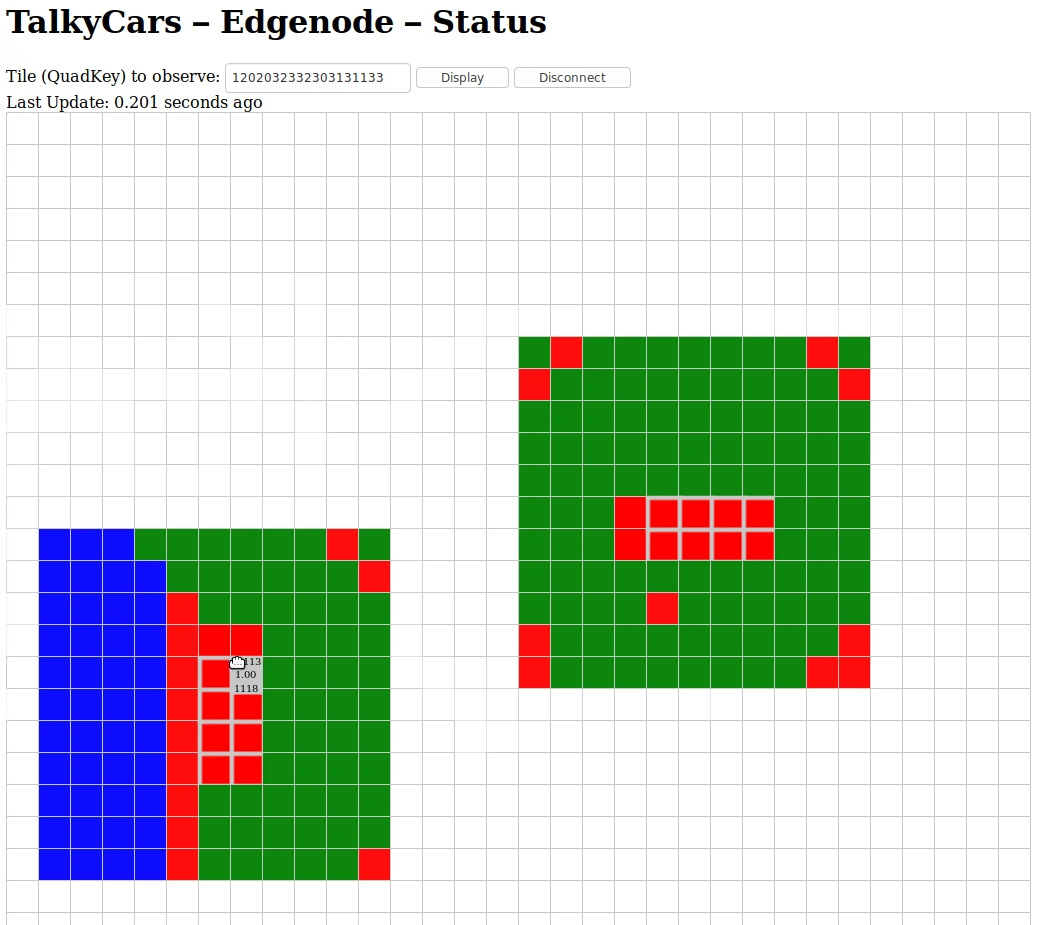
\includegraphics[width=0.8\linewidth]{98_images/screenshot_web_node}
	\caption{Screenshot of an Occupancy Grid's Web Visualization}
	\label{fig:screenshot_web_node}
\end{figure}

\section{On-Board Client-Side Software Components}
\label{sec:implementation:on_board_client_side_software_components}
This section concerns with the implementation of all on-board software components, i.e. modules, which are usually run on an observer device. Usually, such observers will be vehicles, but might be road-side cameras, traffic lights or potentially even pedestrian smartphones as well. All client-side software is implemented in Python and relies on third-party open-source libraries with the following licenses: Apache 2, BSD-3, EPL, LGPL, MIT, MPL. 

\subsection{Simulator Bridge}
\label{subsec:implementation:simulator_bridge}
This first component to run on the client-side, i.e. usually on a vehicle, is specific to this work, as it constitutes a software interface between CP system and simulation environment. In a real-world scenario, a similar component with (ideally) identical interfaces will exist nevertheless. However, it would wrap different functions. Instead of performing API calls to Carla and related data pre-processing it would rather communicate with either the previous AD pipeline module or the vehicle's sensory directly. 

As Carla offers a rich Python API, this component is implemented in Python. As opposed to constituting a stand-alone component, however, it is integrated into the Talky client (see \cref{subsec:implementation:talky_client}) as a collection of encapsulated modules and classes. Following the guidelines for good software architecture presented in \cite{Martin2017} and utilizing appropriate design patterns \cite{EricFreemanElisabethFreemanBertBates2013}, the implementation focuses on establishing a \textbf{strict boundary} between simulation client and Talky client, to make both possibly reusable.

The simulator bridge (or simulation client) communicates to the simulation server via a TCP socket connection and is responsible for performing multiple tasks in interaction with the server:

\begin{itemize}
	\item Offer an interface to control the simulation environment, i.e. frame rate, map, weather conditions, other traffic participants, etc.
	\item Offer an interface to control an ego vehicle
	\item Receive and display rendered images from simulation server
	\item Receive sensor data (via a push mechanism, with a frequency synchronized to the server's tick rate) from the simulation server
	\item Pre-process sensor data
	\item Infer control commands according to a specified behavior or policy
\end{itemize}

\begin{figure}
	\centering
	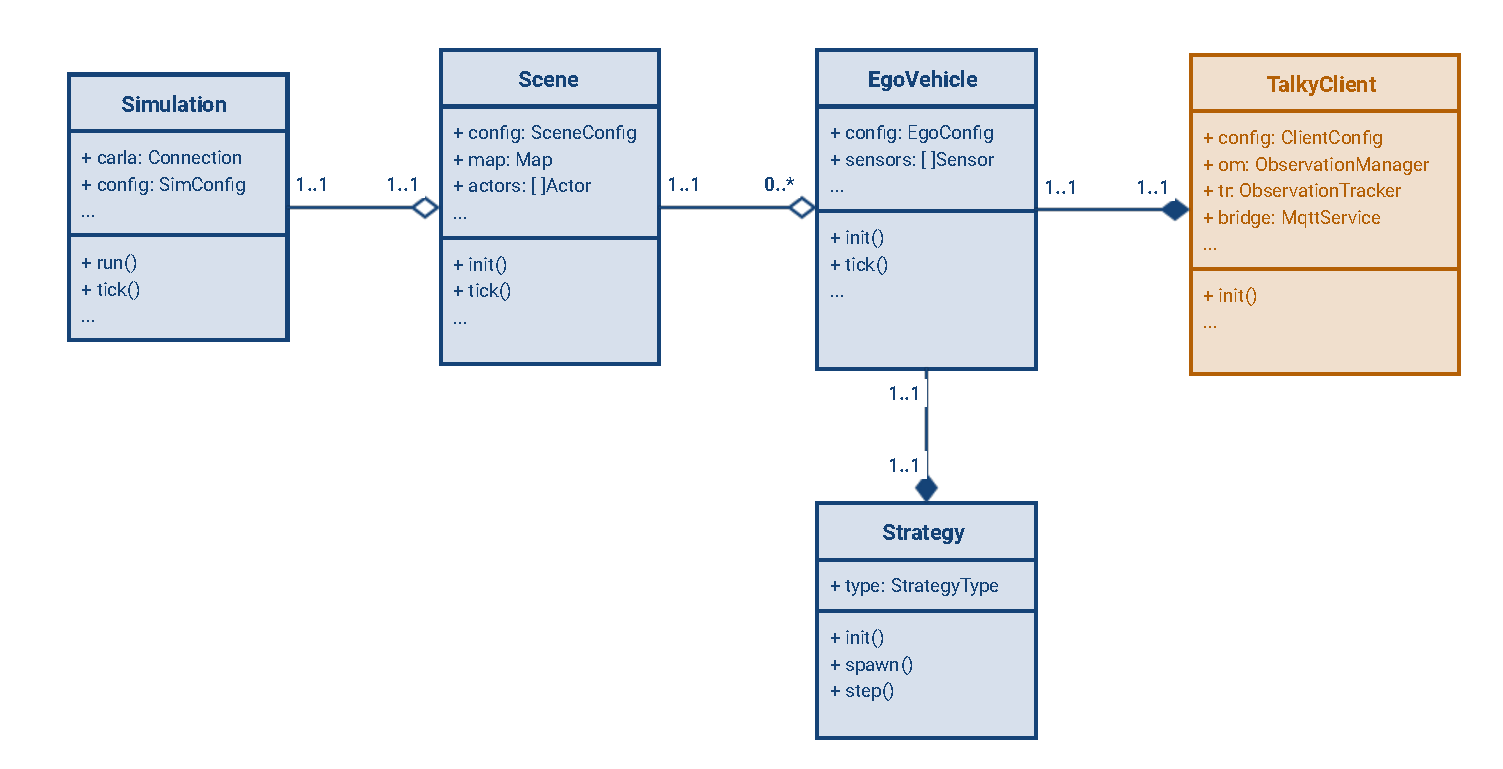
\includegraphics[width=0.9\linewidth]{98_images/client_classes}
	\caption{UML Class Diagram for Simulation Client}
	\label{fig:client_classes}
\end{figure}

\Cref{fig:client_classes} depicts core sub-modules of the simulation client. In order to achieve a high degree of \textbf{modularity} and keep \textbf{clean code boundaries} between simulation-related code and the actual CP system, different abstractions are made.

The \texttt{Simulation} class can be thought of as an entry point to the program. It maintains connection and communication with the Carla server, displays the rendered images and synchronizes client- and server tick rate. Every simulation is initialized with exactly one \texttt{Scene}. It loads the map environment and spawns and controls all "'non-player character"' (NPC) traffic participants, e.g. pedestrians. In addition, it holds references to one or more \texttt{EgoVehicle}s. Each of these represent a connected, intelligent car in the sense of autonomous driving. An ego vehicle, in turn, has access to several sensors, whose data it processes as well as actuators used to control the car. A given behavior, in form of a \texttt{Strategy} instance, specifies how the car interacts with its environment and what "'decision"' it is supposed to take in which situation. Eventually, every ego vehicle holds an instance of exactly one \texttt{TalkyClient}, which corresponds to the respective component presented in \cref{subsec:concept_design:components_overview}. All client-side cooperative perception tasks are performed inside this component and it acts as a bridge to the server-side subsystem via an intermediate MQTT connection with the message broker.

This modular structure enforces a strong \textbf{separation of concerns} and enables for distribution. That is, a certain scene might be hosted on one physical machine, while the contained ego vehicles run on another, e.g. to simulate latency or to better distribute computation load.

\subsection{Talky Client}
\label{subsec:implementation:talky_client}
As mentioned before, this component is one of two core parts of the presented cooperative perception system, together with the \texttt{TalkyEdgeNode} (see \cref{subsec:concept_design:components_overview}). It is implemented in Python and realized as one coherent application together with the simulation client. However, a highly modular structure is followed, so that different parts of the application are re-usable and can be executed separately. Responsibilities of this component include to:

\begin{itemize}
	\item ... compute the current occupancy grid's structure every frame.
	\item ... perform object detection based on received sensor data to derive occupancy states every frame.
	\item ... perform object tracking based on received sensor and derived occupancy states every frame.
	\item ... construct a PER model instance every frame.
	\item ... communicate its local state representation with the server-side fusion at a fixed rate.
\end{itemize}

Particular emphasis is laid on the tasks of detecting and tracking an object in the following. 

In order for a vehicle to construct an occupancy grid model or driveability map, detailed information on all surrounding obstacles is needed. Such include dynamic obstacles, like other traffic participants as well static obstacles, like curbstones, ground-mounted traffic signs, buildings, etc. The first step is to recognize them, also referred to as detection in the following, and a second step is to match and track them. That is, a detected object in one iteration or frame needs to be associated with an instance of itself in subsequent frames. Both problems are subject to current research and only covered in a very basic manner here.
\par
\bigskip

While Carla offers a variety of sensors, including camera and LiDAR, unfortunately, there is no mechanism to directly retrieve all static and dynamic obstacles from the simulation\footnote{\url{https://github.com/carla-simulator/carla/issues/1832}}. Thus, they need to be derived from actual sensor data. For the task of \textbf{detecting} an obstacle, a basic heuristic is applied to  perform \textbf{ray casting} on LiDAR sensor data. LiDAR data usually exists in the form of point clouds, which are, essentially, collections of 3-tuples of world coordinates. For every LiDAR ray, the respective coordinate refers to the point in space where it was reflected, i.e. hit an obstacle. Rays that are not reflected within the sensor's spatial range do not have corresponding triples in the point cloud. Given these data, the two-dimensional position of obstacles in Eucledian space – and thus of occupied cells – can be derived easily. Occupancy cells that do not have a LiDAR collision point falling into them are considered free. However, this indicator is only necessary, but not sufficient for a cell to be considered free. As mentioned in \cref{subsec:concept_design:the_final_model}, the state property is desired to be ternary rather than binary, i.e. distinguish between a cell being occupied or free on the one hand or having an unknown state on the other. Disregarding sensor noise, a cell within the observer's perception range is unknown exactly if no LiDAR ray has a chance to intersect or hit it. These are cells, which are hidden by an obstacle placed between the cell and the sensor. All cells that lie "'behind"' an obstacle, i.e. a cell that contains a LiDAR point, can be considered unknown. On the contrary, all cells "'in front of"' that obstacle can assumed to be free, as the LiDAR ray was able to pass them to eventually hit the target. To determine these cells, a ray casting algorithm is used to check for a ray's intersection with any of the "'boxes"' corresponding to cells between sensor and hit point. The estimation of a cell state can be summarized as follows, given a ray with vector direction $\vec{r_j}$ and magnitude $d_j$:

$$
\textit{state}(cell_i) = 
\begin{cases}
\textit{occupied} & \text{if\ } \textit{contains}(\textit{cell\_box}_i, \langle \vec{r_j}, d_j \rangle) \\
\textit{free} & \text{if\ } \textit{intersects}(\textit{cell\_box}_i, \vec{r_j}) \\
\textit{unknown} & \text{else}
\end{cases}
$$

The implementation of \textit{contains()} is trivial and for \textit{intersects()} the ray casting algorithm shown in \cref{sec:appendix:source_code:ray_casting_intersection_algorithm} was ported to Python. After Python's performance for this algorithm turned out to be comparatively poor, it was re-implemented in Cython\footnote{\url{https://cython.org/}}. Cython is an extension to the Python language and offers support to compile Python-like code to native C code and include it as a module. For computation intense algorithms, this usually improves performance dramatically. In the example of ray casting, the difference in performance between a Python- and C++ implementation of the exact same algorithm can be up to multiple orders of magnitude high \cite{Novak2017}.

It is worth noting that, in a real-world system, object detection would usually be performed by a dedicated pipeline step. Normally, the Talky client would be supplied with already detected obstacles and their positions, which it can infer an occupancy grid from. Thus, the \texttt{OccupancyGridManager}'s matching function would normally take an object list as input, rather than a LiDAR point cloud. The current implementation could easily be adapted to support that by encapsulating the cell matching process in a further sub-module.
\par
\bigskip

The second low-level fusion-related task mentioned above is \textbf{tracking}, which usually goes together with \textbf{matching}. However, for the sake of simplicity and in order to stay within the defined scope, an actual matching mechanism was not implemented. Instead, dynamic objects are identified by their IDs in the simulation. Cells are, trivially, identified by their position, i.e. their QuadKey. Basic tracking is based on the suggestion by \cite{Crowley1993}, the authors of which stated that "'\textit{[n]ewly observed segments enter the model with a low confidence. Successive observations permit the confidence to increase, where as if the segment is not observed in the succeeding cycles, it is considered as noise and removed from the model. Once the system has become confident in a segment, the confidence factor permits a segment to remain in existence for several cycles}"'. Accordingly, a hash map is used to count the number of occurrences of a certain fact, e.g. the state of a specific cell or the presence of a certain car, in subsequent frames. The confidence of the corresponding relation is then set proportionally to its relative presence over the last few (e.g. 10) frames. If it was not seen over a certain number of subsequent frames, it is removed from the hash map and not "'tracked"' anymore. This rudimentary type of tracking was realized as a \texttt{LinearObservationTracker} sub-module and is the central source of confidence values  as fourth parameter in the previously defined model's quadruples.
\par
\bigskip

Communication with the server-side fusion node – via the message broker – is done inside the \texttt{SubscriptionManager} sub-module. On the one hand it acts as an interface for publishing an ego vehicle's current state. On the other hand it maintains according MQTT subscription for type 2- and type 3 tiles (see \cref{subsec:concept_design:geographical_partitioning}), given the ego vehicle's current position. The component holds a reference to an instance of \texttt{MqttBridge} to handle low-level communication. Given this separation, MQTT could be easily switched out by a different publish-subscribe protocol. 

\section{Configurable Parameters}
\label{sec:implementation:configurable_parameters}
In complement to the previous sections, which provided an in-depth description of all involved software components, this section aims to give an overview over relevant parameters, that can be configured by the system's user. They can be categorized into three different classes, depending on which part of the system they affect.

Each of these parameters can be set either through a configuration file or as a program argument.

\subsection{Simulation Parameters}
\label{subsec:implementation:simulation_parameters}
The first set of parameters relates to the simulation.

\begin{figure}
	\centering
	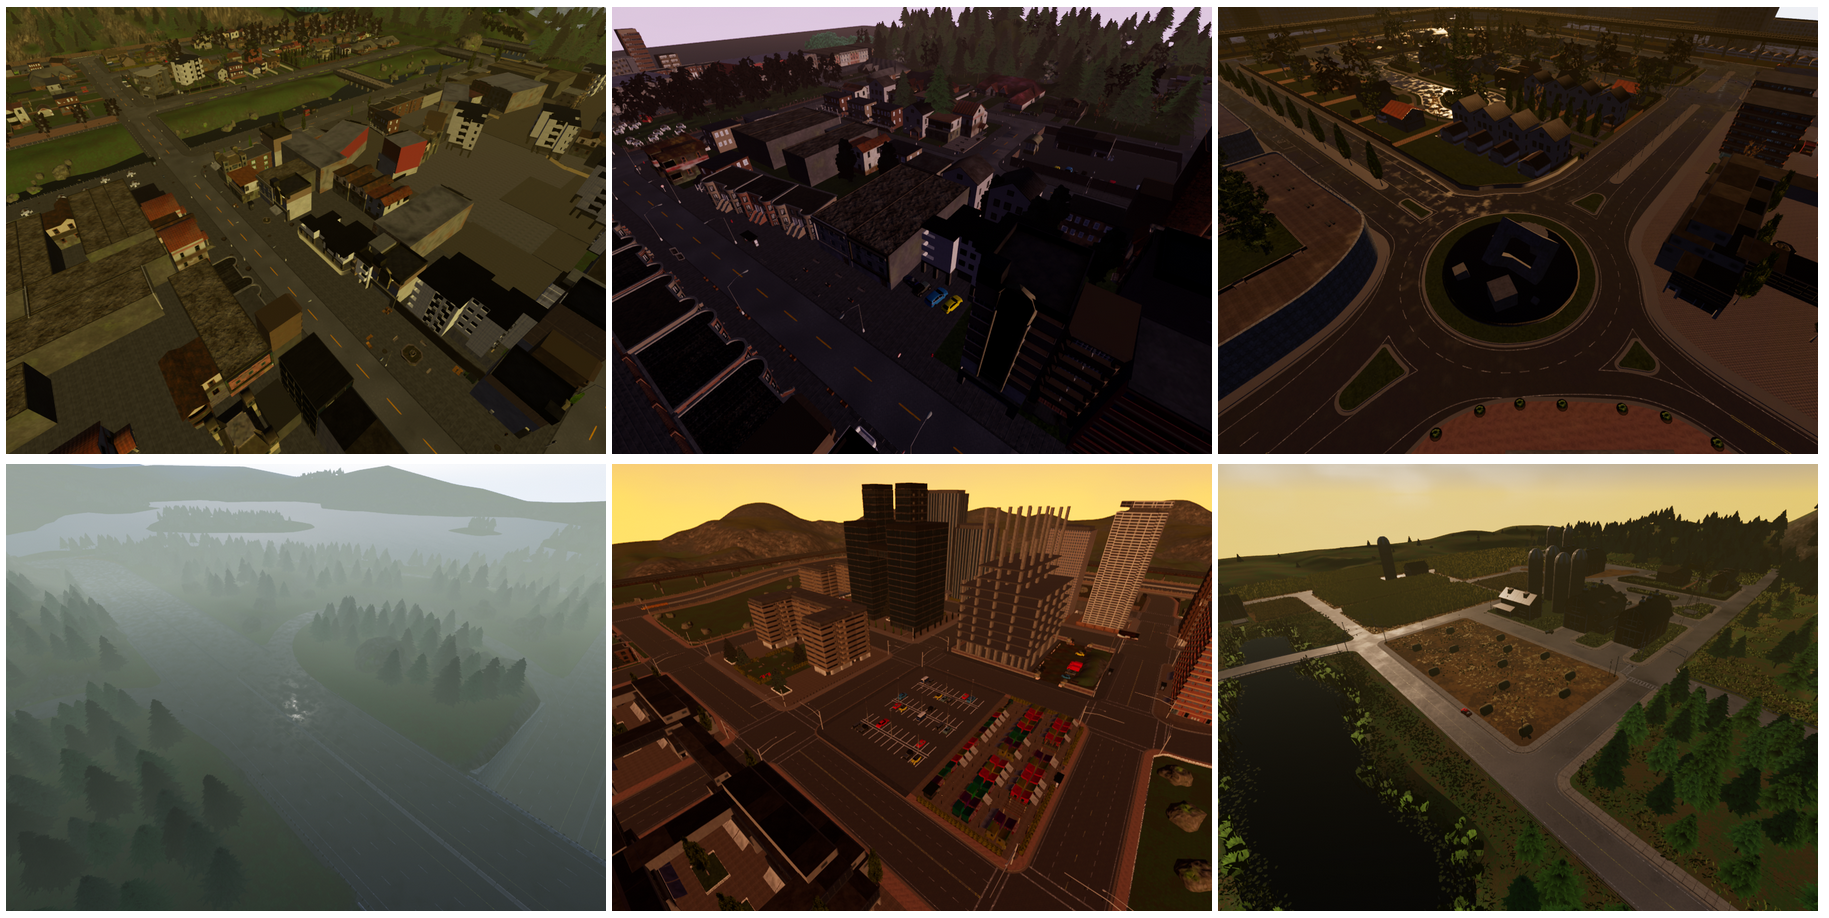
\includegraphics[width=1.0\linewidth]{98_images/carla_collage}
	\caption{Screenshots of Carla Maps}
	\label{fig:carla_collage}
\end{figure}


\begin{table}[H]
	\centering
	\begin{tabular}{|p{7.6cm}|p{7.6cm}|}
		\hline
		\textbf{Parameter} & \textbf{Description} \\ \hline
		\texttt{MAX\_FRAME\_RATE} & Upper bound for the frame rate which to run the simulation at \\ \hline
		\texttt{SENSOR\_\{i\}\_POSITION} & Mounting position of the i-th sensor on the vehicle \\ \hline
		\texttt{LIDAR\_PPS} & Number of points per second sent by LiDAR sensor \\ \hline
		\texttt{LIDAR\_CHANNELS} & Number of vertical LiDAR channels \\ \hline
		\texttt{LIDAR\_ROTATION\_FREQ} & Rotation frequency of the LiDAR sensor \\ \hline
		\texttt{LIDAR\_RANGE} & The LiDAR sensor's range \\ \hline
	\end{tabular}
	\caption{Simulation Parameters}
	\label{tab:simulation_parameters}
\end{table}

\subsection{Scene Parameters}
\label{subsec:implementation:scene_parameters}
The second type of parameters is used to specify details about the current simulation scene.

\begin{table}[H]
	\centering
	\begin{tabular}{|p{7.6cm}|p{7.6cm}|}
		\hline
		\textbf{Parameter} & \textbf{Description} \\ \hline
		\texttt{MAP} & Carla map or environment to run (see \cref{fig:carla_collage}) \\ \hline
		\texttt{N\_NPCS} & Number of "'non-intelligent"' vehicles present in the scene \\ \hline
		\texttt{N\_PEDESTRIANS} & Number of pedestrians present in the scene \\ \hline
		\texttt{N\_EGOS} & Number of connected, intelligent ego vehicles \\ \hline
		\texttt{SPAWN\_POINT\_\{i\}} & Spawn point on the map for the i-th vehicle \\ \hline
		\texttt{SPAWN\_POINT\_POLICY} & Alternatively: A policy for how to choose spawn points \\ \hline
		\texttt{MAX\_SPEED} & Maximum vehicle speed in \si{\km\per\hour} \\ \hline
	\end{tabular}
	\caption{Scene Parameters}
	\label{tab:scene_parameters}
\end{table}

\subsection{Cooperative Perception Parameters}
\label{subsec:implementation:cooperative_perception_parameters}
The last category of parameters refers to such that specify certain aspects of the CP system itself.

\begin{table}[H]
	\centering
	\begin{tabular}{|p{7.6cm}|p{7.6cm}|}
		\hline
		\textbf{Parameter} & \textbf{Description} \\ \hline
		\texttt{TILE\_\{i\}\_LEVEL} & Tile levels to use for geo partitioning \\ \hline
		\texttt{MQTT\_QOS} & MQTT quality of service \\ \hline
		\texttt{OBSERVATION\_MAX\_AGE} & Maximum age (or "'time-to-live"') for an observation to be included in fusion \\ \hline
		\texttt{FUSION\_RATE} & Rate at which to perform fusion (server-side) \\ \hline
		\texttt{OBSERVATION\_RATE} & Rate at which to publish observations (client-side) \\ \hline
		\texttt{DECAY\_FACTOR} & Exponential factor for temporal decay \\ \hline
	\end{tabular}
	\caption{Cooperative Perception Parameters}
	\label{tab:cooperative_perception_parameters}
\end{table}

\section{Open-Source Contributions}
\label{sec:implementation:open_source_contributions}
The present project heavily relies on third-party open-source libraries without which the implementation would not have been possible in this form. Therefore, the efforts taken by the community are highly appreciated. Moreover, code contributions to several open-source projects have been made on the course of this thesis. Such include the Carla project\footnote{\url{https://github.com/carla-simulator/carla}}, \texttt{buckhx/tiles}\footnote{\url{https://github.com/buckhx/tiles}}, a QuadKey implementation for Go, \texttt{buckhx/QuadKey}\footnote{\url{https://github.com/buckhx/QuadKey}}, a QuadKey implementation for Python (later \texttt{n1try/pyquadkey2}\footnote{\url{https://github.com/n1try/pyquadkey2}}), \texttt{ethlo/jquad}\footnote{\url{https://github.com/ethlo/jquad}}, a QuadKey implementation for Java and \texttt{johnnovak/raytriangle-test}\footnote{\url{https://github.com/johnnovak/raytriangle-test}}, a benchmark of ray casting in different programming languages.

\section{Summary}
\label{sec:implementation:summary}
This chapter discussed details about the concrete implementation of concepts and components presented in \cref{ch:concept_design}. The resulting software is subsequently evaluated in \cref{ch:evaluation} and constitutes an exemplary proposal for a novel, holistic cooperative perception system.

In order to use it in real-world scenarios, one would have to add thorough quality assurance and testing as well as various performance optimizations. However, since the system is built following a modular approach it is comparatively easy to re-use or replace certain parts, while keeping others. Accordingly, the simulation client, for instance, might be switched out by a component interfacing with a real AD pipeline without too much effort. As this implementation is published as an open-source project\footnote{\url{https://github.com/n1try/talkycars-thesis}}, it can be used openly as a based for further research. 